\begin{figure}[t]
    \centering
    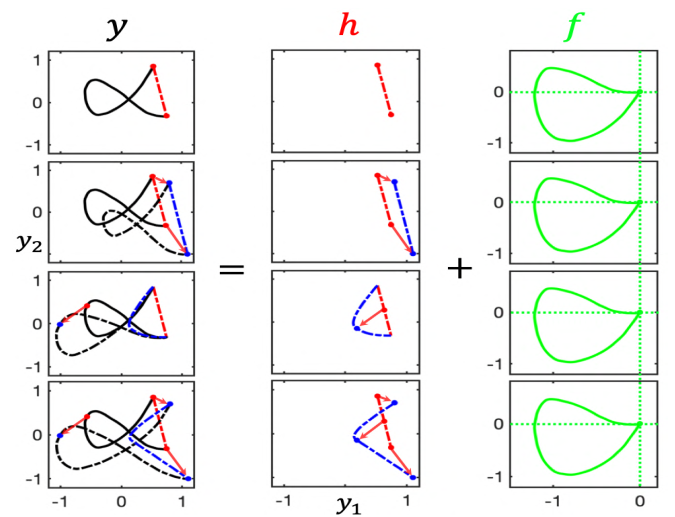
\includegraphics[width=0.7\textwidth]{figures/images/vmp/vmp.png}
    \caption{Graphical representation of the idea behind VMP \cite{zhou2019learning}. The final trajectory \( y \) is represented as the sum of two components: the elementary trajectory \( h \), and the shape modulation \( f \). The elementary trajectory can directly connect two points (e.g., start and goal points) with a linear segment.}
    \label{fig:vmp}
\end{figure}
